\documentclass[class=article, crop=false]{standalone}
\usepackage{tikz}
\usepackage{subcaption}
\usetikzlibrary{calc}

\begin{document}
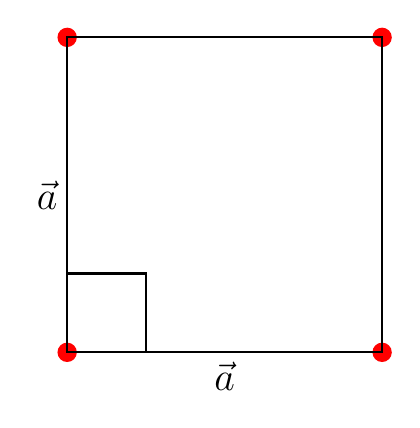
\begin{tikzpicture}
    \def\a{4}  % length of side a

    % Calculate the coordinates of the points
    \coordinate (A) at (0, 0);
    \coordinate (B) at (\a, 0);
    \coordinate (C) at (\a, \a);
    \coordinate (D) at (0, \a);

    \fill[red]  (A) circle(3.5pt) (B) circle(3.5pt) (C) circle(3.5pt) (D) circle(3.5pt);

    % Draw the square unit cell
    \draw[thick] (A) -- (B) -- (C) -- (D) -- cycle;

    % Draw right angle
    \draw[thick] (0,1) -- (1,1) -- (1,0);

    %Draw lattice parameters
    \node[left] at ($(A)!0.5!(D)$) {\Large $\vec{a}$};
    \node[below] at ($(A)!0.5!(B)$) {\Large $\vec{a}$};
    
\end{tikzpicture}
\end{document}